%\documentclass[compress,dvips,xcolor=table]{beamer}
\usepackage{etex}
%\documentclass{article}
%\usepackage{beamerarticle}
%\usepackage[turkish]{babel}
\usepackage[utf8]{inputenc}
\usepackage{tikz}
\usetikzlibrary{shapes,arrows,positioning,calc,shadows,matrix,fit}
\usepackage[graph,arrow,curve,color]{xy}
\usepackage{listings}
\usepackage{multicol}
%\includeonlyframes{current}

\def\circtxt#1{$\mathalpha \bigcirc \mkern-13mu \mathtt #1$}

\mode<article>
{
  \usepackage{fullpage}
  \usepackage{pgf}
  \usepackage{hyperref}
}

\mode<presentation>
{
  \usetheme{metuceng}

%  \setbeamercovered{transparent}
}


\title{Programming Language Concepts}
\subtitle{Binding and Scope}
\author{Onur Tolga Şehitoğlu}
\institute[ODTÜ]{Bilgisayar Mühendisliği}
\subject{Binding and Scope}
\date{}
	\titlegraphic{\insertmetutitle\insertlicense}


\begin{document}
\lstset{language=C,
        basicstyle=\scriptsize\ttfamily,
        keywordstyle=\color{blue!50!black}\bfseries,
        identifierstyle=\color{blue!60!green}\sffamily,
        stringstyle=\color{red!70!green}\ttfamily,
	commentstyle=\color{blue!30!white}\itshape,
        showstringspaces=true}
\setbeamercolor{hexample}{bg=green!5!white,fg=black}%
\setbeamercolor{cexample}{bg=blue!5!white,fg=black}%
\setbeamercolor{pexample}{bg=orange!5!white,fg=black}%
\setbeamercolor{oexample}{bg=violet!5!white,fg=black}%

 \frame[plain]{\maketitle}
 \begin{frame}
 \frametitle{Outline}
 \begin{multicols}{2}
 \tableofcontents
 \end{multicols}
 \end{frame}

\section{Abstraction}
\begin{frame}
\frametitle{Abstraction}
\begin{columns}
 \begin{column}{.3\linewidth}
  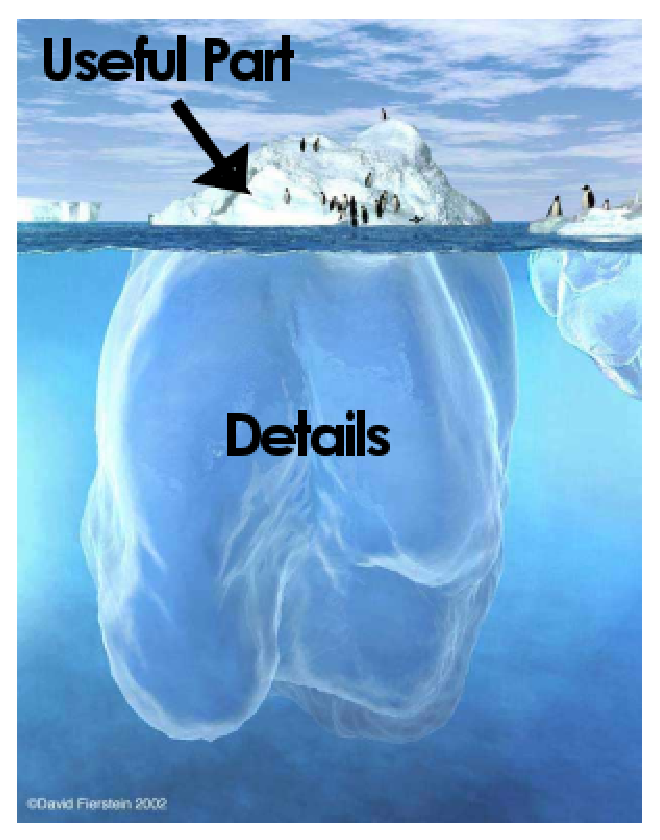
\includegraphics[width=\linewidth]{iceberg}
 \end{column}
\begin{column}{.7\linewidth}
\begin{itemize}[<+->]
\item Iceberg: Details at the bottom, useful part at the top of the ocean. Animals do not care
about the bottom.
\item User: ``how do I use it?'', Developer: ``How do I make it work?''
\item User: ``what does it do?'', Developer: ``How does it do that?
\end{itemize}
\end{column}
\end{columns}
\begin{itemize}
\item \structure{Abstraction:} Make a program or design reusable by enclosing it in a body,
hiding the details, and defining a mechanism to access it.
\item Separating the usage and implementation of program segments.
\item Vital large scale programming.
\end{itemize}
\end{frame}

\begin{frame}
 \begin{itemize}[<+->]
  \item Abstraction is possible in any discipline involving design:
  \item radio tuner. Adjustment knob on a radio is an abstraction over the
  tuner element, frequency selection.
 \item An ATM is an abstraction over complicated set of bank transaction operations.
 \item Programming languages can be considered as abstraction over machine language.
 \item ...
 \end{itemize}
\end{frame}

\begin{frame}
 \frametitle{Purpose}
 \begin{itemize}[<+->]
  \item Details are confusing
  \item Details may contain more error
  \item Repeating same details increase complexity and errors
  \item Abstraction philosophy: \structure{Declare once, use many times!}
  \item \structure{Code reusability} is the ultimate goal.
  \item Parameterization improves power of abstraction
 \end{itemize}
\end{frame}

\subsection{Function and Procedure Abstractions}
\begin{frame}
\frametitle{Function and procedure abstractions}
\begin{itemize}[<+->]
 \item The computation of an expression is the detail (algorithm, variables, etc.)
 \item Function call is the usage of the detail
 \item Functions are \structure{abstractions over expressions}
 \item \texttt{void} functions of C or  \textsf{procedure} declarations of some languages
 \item No value but contains executable statements  as detail.
 \item Procedures are  \structure{abstractions over commands}
 \item Other type of abstractions possible?
\end{itemize}
\end{frame}

\subsection{Selector Abstraction}
\begin{frame}[fragile]
\frametitle{Selector abstraction}
\begin{itemize}[<+->]
 \item arrays: \texttt{ int a[10][20];  a[i]=a[i]+1;}
 \item \texttt{ [..] } operator selects elements of an array.
 \item User defined selectors on user defined structures?
 \item Example: Selector on a linked list:
\begin{beamercolorbox}{cexample}\noindent
\begin{lstlisting}[language={C++},escapechar=\#]
struct List {
  int data;
  List *next;
  int & operator[](int el) {
    int i; List *p = this;
    for (i = 1 ; i < el ; i++) 
      p = p->next;       /* take the next element */
    return p->data;
  };
  ...
};
List h;
...
h[1] = h[2] + 1;
\end{lstlisting}
\end{beamercolorbox}
\item C++ allows overloading of \texttt{[]} operator for classes.
\end{itemize}
\end{frame}

\begin{frame}[fragile]
\begin{itemize}
\item {\small Python \lstinline[language=Python]{__setitem__(k,v)} implements l-value,
\lstinline[language=Python]{__getitem__(k)} r-value selector.}
\end{itemize}
\begin{beamercolorbox}{pexample}\noindent
\begin{lstlisting}
class BSTree:
  def __init__(self):
    self.node = None
  def __getitem__(self, key):
    if self.node == None:
        raise KeyError
    elif key < self.node[0]: return self.left[key]
    elif key > self.node[0]: return self.right[key]
    else:                    return self.node[1]
  def __setitem__(self, key, val):
    if self.node == None:
        self.node = (key,val)
        self.left = BSTree()    # empty tree
        self.right = BSTree()   # empty tree
    elif key < self.node[0]: self.left[key] = val
    elif key > self.node[0]: self.right[key] = val
    else:                    self.node = (key,val)

a = BSTree()
a["hello"] = 4
a["world"] = a["hello"] + 5
\end{lstlisting}
\end{beamercolorbox}
\end{frame}

\begin{frame}[fragile]
\begin{beamercolorbox}{cexample}
\begin{lstlisting}[language=C++]
class BST {
    struct Node { string key; double val; 
                  Node *left, *right;} *node;
public:
    BST() { node = NULL;};
    double & operator[](const string &k) {
        Node **parent = NULL, *p = node, *newnode;
        while (p != NULL) {
            if (k < p->key) {
                parent = &p->left; p = p->left;
            } else if (k > p->key) {
                parent = &p->right; p = p->right;
            } else return p->val;
        }
        newnode = new Node;
        newnode->left = newnode->right = NULL;
        newnode->key = k; 
        if (parent == NULL) node = newnode;
        else                *parent = newnode;
        return newnode->val;
   }
};
BST a;
a["carrot"] = 3; a["onion"] = 4;
a["patato"] = a["onion"] + 2;
\end{lstlisting}
\end{beamercolorbox}
\end{frame}

\defverbatim[colored]\codetemplateCpp{
\begin{lstlisting}[language={C++},escapechar=\#]
template <class #\alert{T}#>
  class List {
	#\alert{T}# content;
	List *next;
  public: List() { next=NULL };
	void add(#\alert{T}# el) { ... };
	#\alert{T}# get(int n) { ...};
  };
template <class #\alert{U}#>
  void swap(#\alert{U}# &a, #\alert{U}# &b) { #\alert{U}# tmp; tmp=a; a=b; b=tmp; }
...
List<#\alert{int}#> a; List<#\alert{double}#> b; List<#\alert{Person}#> c;
int t,x; double v,y; Person z,w;
swap(t,x); swap(v,y); swap(z,w);
\end{lstlisting}}
\subsection{Generic Abstraction}
\begin{frame}
\frametitle{Generic abstraction}
\begin{itemize}
 \item Same declaration pattern applied to different data types.
 \item \structure{Abstraction over declaration}. A function or class declaration can be adapted
 to different types or values by using type or value parameters.
\begin{beamercolorbox}{cexample}
 \codetemplateCpp
\end{beamercolorbox}
\end{itemize}
\end{frame}

\defverbatim[colored]\codeiteratorabsRuby{
\begin{lstlisting}[language={Ruby},escapechar=\~]
class Tree
   def initialize(v)
        @value = v ; @left = nil ; @right = nil
   end
   def traverse
        @left.traverse  {|v| yield v}  if @left != nil
        yield @value        # block argument replaces
        @right.traverse {|v| yield v}  if @right != nil
   end
end

a=Tree.new(3) ; l=[]
a.traverse { |node|	  # yield  param
	     print node   # yield body
             l << node    # yield body
	   }
\end{lstlisting}}
\subsection{Iterator Abstraction}
\begin{frame}
\frametitle{Iterator abstraction}
\begin{itemize}
\item Iteration over a user defined data structure. \structure{Ruby} example:
\begin{beamercolorbox}{oexample}
 \codeiteratorabsRuby
\end{beamercolorbox}
\end{itemize}
\end{frame}

\defverbatim[colored]\codeiteratorabsPython{
\begin{lstlisting}[language={Python},escapechar=\~]
class BSTree(object):
    def __init__(self):
            self.val = ()
    def inorder(self):
        if self.val == ():
            return
        else:
            for i in self.left.inorder():
                yield i
            yield self.val
            for i in self.right.inorder():
                yield i
v = BSTree()
...
for v in v.inorder():
    print v
\end{lstlisting}}
\subsection{Iterator Abstraction}
\begin{frame}
\frametitle{Iterator abstraction}
\begin{itemize}
\item Iteration over a user defined data structure. \structure{Python} generator example:
\begin{beamercolorbox}{oexample}
 \codeiteratorabsPython
\end{beamercolorbox}
\end{itemize}
\end{frame}

\begin{frame}[fragile]
\frametitle{C++ iterators}
\begin{itemize}
\item C++ Standard Template Library containers support \structure{iterators}
\item \lstinline!begin()! and \lstinline!end()! methods return iterators to start and end of the data structure
\item Iterators can be dereferenced as \lstinline!*iter! or \lstinline!iter->member!.
\item `\lstinline!++!' operation on an iterator skips to the next value.
\item \begin{lstlisting}[language=C++,escapeinside=`']
for (`\em ittype\/' it = a.begin(); it != a.end(); ++it) {
    // use *it or it->member it->method() in body
}
\end{lstlisting}
\item C++11 added:
\begin{lstlisting}[language=C++,escapeinside=`']
for (`\em valtype\/' & i : a ) {
    // use directly i as l-value or r-value. 
}
\end{lstlisting}
This syntax is equivalent to:
\begin{lstlisting}[language=C++,escapeinside=`']
for (`\em ittype\/' it = a.begin() ; it != a.end(); it++) {
    `\em valtype\/' & i = *it;
    // use directly i as l-value or r-value 
}
\end{lstlisting}
\end{itemize}
\end{frame}

\begin{frame}[fragile]
\frametitle{C++ iterators}
\begin{beamercolorbox}{cexample}
\begin{lstlisting}[language=C++]
template<class T> class List {
  struct Node { T val; Node *next;} *list;
public: List() { list = nullptr;}
  void insert(const T& v) { Node *newnode = new Node;
      newnode->next =list; newnode->val = v; list = newnode;}
  class Iterator {
    Node *pos;
  public: Iterator(Node *p) { pos = p;}
    T & operator*() { return pos->val; }
    void operator++() { pos = pos->next; }
    bool operator!=(const Iterator &it) { return pos != it.pos; }
  };
  Iterator begin() { Iterator it = Iterator(list); return it; }
  Iterator end() { Iterator it = Iterator(nullptr); return it; }
};
...
List<int> a;
// C++11 syntax below
for (int & i : a ) {  i *= 2; cout << i << '\n'; }
for (const char * s : { "ankara","istanbul","izmir" }) { 
    cout << s ; }
\end{lstlisting}
\end{beamercolorbox}
\end{frame}


\section{Abstraction Principle}
\begin{frame}
 \frametitle{Abstraction Principle}
\begin{itemize}
 \item If any programming language entity involves computation, it is possible to define an
abstraction over it\\

\rowcolors[]{1}{blue!5!white}{blue!5!white}
\begin{tabular}{l!{$\rightarrow$}l}\rowcolor{blue!10!white}
 \bf Entity & \bf Abstraction \\
 Expression	& Function \\
 Command  & Procedure \\
 Selector & Selector function \\
 Declaration  & Generic \\
 Command Block & Iterator \\
\end{tabular}
\end{itemize}
\end{frame}

\section{Parameters}
\begin{frame}
\frametitle{Parameters}
\begin{itemize}[<+->]
 \item Many purpose and behaviors in order to take advantage of ``declare once use many times''.
 \item \textbf{Declaration part:}
	\texttt{abstraction\_name(Fp$_1$, Fp$_2$, ..., Fp$_n$) } \\
       \textbf{Use part:}
	\texttt{abstraction\_name(Ap$_1$, Ap$_2$, ..., Ap$_n$) } 
 \item Formal parameters: identifiers or constructors of identifiers (patterns in functional
languages)
 \item Actual parameters: expression or identifier based on the type of the abstraction and
parameter
 \item \alert{Question:} How actual and formal parameters relate/communicate?
 \item Programming language design should answer
 \item \structure{Parameter passing mechanisms}
\end{itemize}
\end{frame}

\section{Parameter Passing Mechanisms}
\begin{frame}
\frametitle{Parameter Passing Mechanisms}
 Programming language may support one or more mechanisms. 3 basic methods:
\begin{enumerate}
 \item Copy mechanisms (assignment based)
 \item Binding mechanisms 
 \item Pass by name (substitution based)
\end{enumerate}
\end{frame}

\subsection{Copy Mechanisms}
\begin{frame}
\frametitle{Copy Mechanisms}
\begin{itemize}[<+->]
 \item Function and procedure abstractions, assignment between actual and formal parameter:
\begin{enumerate}
 \item \structure{Copy In:} \\
	On function call: $Fp_i \leftarrow Ap_i$
 \item \structure{Copy Out:} \\
	On function return: $Ap_i \leftarrow Fp_i$
 \item \structure{Copy In-Out:} \\
	On function call: $Fp_i \leftarrow Ap_i$, and\\
	On function return: $Ap_i \leftarrow Fp_i$
\end{enumerate}
 \item C only allows copy-in mechanism. This mechanism is also called as \structure{Pass by value}.
\end{itemize}
\end{frame}

\defverbatim[colored]\codeparpassC{
\begin{lstlisting}[language={C},escapechar=\#]
int x=1, y=2;
void f(int a, int b) {
    x += a+b;
    a++;
    b=a/2;
}
int main() {
    f(x,y);
    printf("x:%d , y:%d\n",x,y);
    return 0;
}
\end{lstlisting}}
\begin{frame}
\begin{columns}
 \begin{column}{.55\linewidth}
  \begin{beamercolorbox}{cexample}
  \codeparpassC
  \end{beamercolorbox}
 \end{column}
\begin{column}{.45\linewidth}\scriptsize
\only<1-1>{
 \underline{\structure{Copy In:}}\\
 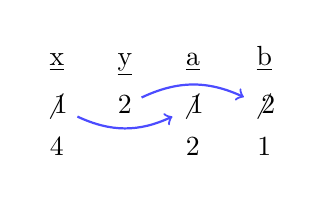
\begin{tikzpicture}
	\matrix [matrix of nodes,nodes in empty cells,ampersand replacement=\&,column sep=4mm] (m) {
  		\underline{x} \&\underline{y} \&\underline{a} \&\underline{b} \\
  		   {$\not 1$} \& {$2$} \& {$\not 1$} \& {$\not 2$} \\ 
  $4$ \&  \&  $2$ \& $1$ \\
	};
	\draw [bend right=25,->,thick,blue!70!white] (m-2-1) to (m-2-3); 
	\draw [bend left=25,->,thick,blue!70!white] (m-2-2) to (m-2-4); 
 \end{tikzpicture}\ \\
\texttt{x:4, y:2}\\}
\only<2-2>{
\underline{\structure{Copy Out:}}\\
 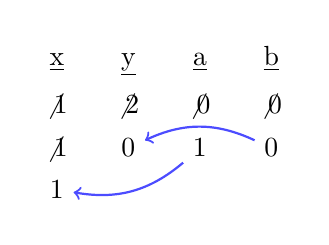
\begin{tikzpicture}
	\matrix [matrix of nodes,nodes in empty cells,ampersand replacement=\&,column sep=4mm] (m) {
  \underline{x} \&\underline{y} \&\underline{a} \&\underline{b} \\
  $\not 1$ \& $\not 2$ \& $\not 0$ \& $\not 0$ \\
  $\not 1$      \&  {$0$}   \& {$1$}  \& {$0$} \\
  {$1$} \& \& \& \\ 
 };
	\draw [bend left=25,->,thick,blue!70!white] (m-3-3) to (m-4-1); 
	\draw [bend right=25,->,thick,blue!70!white] (m-3-4) to (m-3-2); 
\end{tikzpicture}\ \\
\texttt{x:1, y:0}\\}
\only<3-3>{
\underline{\structure{Copy In-Out:}}\\
 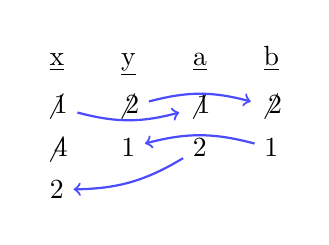
\begin{tikzpicture}
	\matrix [matrix of nodes,nodes in empty cells,ampersand replacement=\&,column sep=4mm] (m) {
  \underline{x} \&\underline{y} \&\underline{a} \&\underline{b} \\
  {$\not 1$} \& {$\not 2$} \& {$\not 1$} \& {$\not 2$} \\ 
  $\not 4$ \&  {$1$}\&  {$2$} \& {$1$} \\
  {$2$} \\
};
	\draw [bend right=15,->,thick,blue!70!white] (m-2-1) to (m-2-3); 
	\draw [bend left=15,->,thick,blue!70!white] (m-2-2) to (m-2-4); 
	\draw [bend left=15,->,thick,blue!70!white] (m-3-3) to (m-4-1); 
	\draw [bend right=15,->,thick,blue!70!white] (m-3-4) to (m-3-2); 
\end{tikzpicture}\ \\
\texttt{x:2, y:1}\\}
\end{column}
\end{columns}
\end{frame}

\subsection{Binding Mechanisms}
\begin{frame}
\frametitle{Binding Mechanisms}
 \begin{itemize}
  \item  Based on binding of the formal parameter variable/identifier to actual parameter
value/identifier.
  \item Only one entity (value, variable, type) exists with more than one names.
\begin{enumerate}
  \item \structure{Constant binding:} Formal parameter is constant during the function. The
value is bound to actual parameter expression value. \\
  Functional languages including Haskell uses this mechanism.
  \item \structure{Variable binding:} Formal parameter variable is bound to the actual
parameter variable. Same memory area is shared by two variable references.\\
  Also known as \structure{pass by reference} \\
\end{enumerate}
  \item The other type and entities (function, type, etc) are passed with similar mechanisms. 
\end{itemize}
\end{frame}


\begin{frame}
\begin{columns}
 \begin{column}{.55\linewidth}
  \begin{beamercolorbox}{cexample}
  \codeparpassC
  \end{beamercolorbox}
 \end{column}
\begin{column}{.45\linewidth}\small
 \underline{\structure{Variable binding:}}\\
 \begin{tabular}{cp{.5em}c}
  \only<2-2>{f():a /} & & \only<2-2>{f():b /} \\
  x & & y \\ \cline{1-1} \cline{3-3}
   $\not 1$ 		& &  	$\not 2$	\\
   $\not 4$ 		& &  	$2$	\\
   $5$ 			& &  		\\
 \end{tabular}\\
\only<3-3>{\texttt{x: 5, y:2}}
\end{column}
\end{columns}
\end{frame}

\defverbatim[colored]\codefonkH{
\begin{lstlisting}[language={Haskell}]
f x y = if (x<12) then x*x+y*y+x 
                  else x+x*x
\end{lstlisting}}
\subsection{Pass by Name}
\begin{frame}
\frametitle{Pass by name}
\begin{itemize}
 \item Actual parameter syntax replaces each occurence of the formal parameter in the function
body, then the function body evaluated.
 \item C macros works with a similar mechanism (by pre-processor)
 \item Mostly useful in theoretical analysis of PL's. Also known as
 \structure{Normal order evaluation}
 \item Example (Haskell-like)\\
\begin{beamercolorbox}{hexample}
\codefonkH
\end{beamercolorbox}
  Evaluation:
  \texttt{\scriptsize f (3*12+7) (24+16*3) $\mapsto$
	  if ((3*12+7)<12) then (3*12+7)*(3*12+7)+(24+16*3)*(24+16*3)+(3*12+7) 
                  else (3*12+7)+(3*12+7)*(3*12+7) $\stackrel{*}{\mapsto}$
	if (43<12) then ... $\mapsto$
        if (false) then ... $\mapsto$ (3*12+7)+(3*12+7)*(3*12+7) $\stackrel{*}{\mapsto}$
	(3*12+7)+43*(3*12+7) $\mapsto$ ... $\mapsto$ 1892} \hfill \structure{\small\rm (12 steps)}
\end{itemize}
\end{frame}

\section{Evaluation Order}
\begin{frame}
\frametitle{Evaluation Order}
\begin{itemize}
\item \structure{Normal order evaluation} is mathematically natural order of evaluation.
\item Most of the PL's apply \structure{eager evaluation}: Actual parameters are evaluated
first, then passed.\\
\texttt{\scriptsize f (3*12+7) (24+16*3) $\mapsto$
	f (36+7) (24+16*3) $\stackrel{*}{\mapsto}$
	f 43 72 $\mapsto$  if (43<12) then 43*43+72*72+43 
                  else 43+43*43 $\mapsto$ if (false) then ... $\mapsto$
	43+43*43 $\stackrel{*}{\mapsto}$ 1892}\hfill \structure{\small\rm (8 steps)}
\item Consider ``\lstinline!g x y= if x>10 then y else x!"  for \texttt{g 2 (4/0)}
\item Side effects are repeated in NOE.
\item \structure{Church–Rosser Property:} {\small\rm
If an expression can be evaluated at all, it can be evaluated by consistently using
normal-order evaluation. If an expression can be evaluated in several different orders
(mixing eager and normal-order evaluation), then all of these evaluation orders yield
the same result.}
\end{itemize}
\end{frame}

\begin{frame}
In $\lambda$-calculus, all orders reduce the same normal form.\\
\tiny
\xygraph{[]!{<14mm,0mm>:<0mm,8mm>::}
{\lambda x.(\lambda y.y+(\lambda x.x+1~y)~~(x+2))~~5}
 ( :@{|->}[dll] {\lambda y.y+(\lambda x.x+1~~y)~~(5+2)}
    ( :@{|->}[dl] {5+2+(\lambda x.x+1~~(5+2))}
        ( :@{|->}[ddddrrr] {5+2+5+2+1}="bot" ) ,
      :@{|->}@(dr,ur)[dddl] {\lambda y.y+y+1~~(5+2)} :@{|->}"bot"
    ),
   :@{|->}[dd]  {\lambda x.x+2+(\lambda x.x+1~~(x+2))~5}
    (
    :@{|->}[dl]  {5+2+(\lambda x.x+1~~(5+2))} :@{|->}"bot",
    :@{|->}[dr]  {\lambda x.x+2+x+2+1~~5} :@{|->}"bot"
    ),
   :@{|->}[drr] {\lambda x.(\lambda y.y+y+1~~(x+2))~~5} (
       :@{|->}[ddr] {\lambda y.y+y+1~~(5+2)} :@{|->}@(dr,r)"bot",
       :@{|->}[ddd] {\lambda x.x+2+x+2+1~~5} :@{|->}"bot")
 )
}
\end{frame}


\begin{frame}
\begin{itemize}
\item Haskell implements \structure{Lazy Evaluation } order.
\item Eager evaluation is faster than normal order evaluation but violates Church-Rosser
Property. Lazy evaluation is as fast as eager evaluation but computes same results with normal
order evaluation (unless there is a side effect)
\item Lazy evaluation expands the expression as normal order evaluation however once it
evaluates the formal parameter value other evaluations use previously found value:\\
\texttt{\scriptsize f (3*12+7) (24+16*3) $\mapsto$
	  if (x:(3*12+7)<12) then x:(3*12+7)*x:(3*12+7)+y:(24+16*3)*y:(24+16*3)+x:(3*12+7) 
                  else x:(3*12+7)+x:(3*12+7)*x:(3*12+7) $\stackrel{*}{\mapsto}$
	if (x:43<12) then x:43*x:43+y:(24+16*3)*y:(24+16*3)+x:43
                  else x:43+x:43*x:43 $\mapsto$ if (false) then ... $\mapsto$ x:43+x:43*x:43
	$\mapsto$ x:43+1849 $\mapsto$ 1892}\hfill \structure{\small\rm (7 steps)}
	

\end{itemize}
\end{frame}

\begin{frame}[fragile]
\frametitle{Lazy Evaluation}
\small
\begin{itemize}
\item Parameters are passed by name but compiler keeps evaluation state of them. Parameter value is store once it is evaluated. Further evaluations use that.
\item Python implementation. First delay evaluation of expressions. Convert to functions:\\
\lstinline!exp! $\rightarrow$ \lstinline[language=Python]!lambda : exp! \\
$\eta$ expansion. Function version is also called \structure{thunk}.
\item Inside function, call these functions to evaluate the expression.
\begin{beamercolorbox}{pexample}
\begin{lstlisting}[language=Python,basicstyle=\tiny\tt]
def E(thunk):
  if not hasattr(thunk,"stored"):
    thunk.stored = thunk()      # evaluate and store
  return thunk.stored           # use stored value

def f(x,y):
  if E(x) < 10:                # call E() on all evaluations
    return E(x)*E(x)+E(y)
  else:
    return E(x)*E(x)+E(x)

f(lambda : 3*32+4, lambda: 4/0)     # call by converting to function
\end{lstlisting}
\end{beamercolorbox}
\end{itemize}
\end{frame}

\section{Infinite Values}
\begin{frame}[fragile]
\frametitle{Infinite Values}
\begin{itemize}
\item Delayed evaluation in normal order or lazy evaluation enables working on infinite values:
\begin{beamercolorbox}{hexample}
\begin{lstlisting}[language=Python]
take _ [] = []
take n (a:r) | n == 0 = []
             | otherwise = a : take (n-1) r
x = (1:2:x)
\end{lstlisting}
\texttt{\scriptsize take 3 x $\mapsto$ take 3 (1:2:x) $\mapsto$ 1:take (3-1) (2:x) $\mapsto$ \\
1:2:take (2-1) x $\mapsto$ 1:2:take 1 (1:2:x) $\mapsto$ 1:2:1:take (1-1) (2:x)
$\mapsto$ 1:2:1:[]}
\end{beamercolorbox}
\item Programmers can take advantage of this. Construct an infitely value, take as many as program needs. For example expand $\pi$ in an infinite value, stop when desired resolution achieved.
\end{itemize}
\end{frame}

\section{Correspondence Principle}
\begin{frame}
\frametitle{Correspondence Principle}
\begin{itemize}
\item \structure{Correspondence Principle}:\\
	 For each form of declaration there exists a corresponding parameter mechanism.
\item C:\\
\rowcolors[]{2}{blue!5!white}{blue!10!white}
\begin{tabular}{>{\tt}l!{$\leftrightarrow$}>{\tt}l}\rowcolor{blue!5!white}
int a=p; & void f(int a) \{ \\
const int a=p;  & void f(const int a) \{ \\
\end{tabular}
\item Pascal:\\
\rowcolors[]{2}{blue!5!white}{blue!10!white}
\begin{tabular}{>{\tt}l!{$\leftrightarrow$}>{\tt}l}\rowcolor{blue!5!white}
var a: integer; & procedure f(a:integer) begin \\
const a:5;  & ??? \{ \\
???	    & procedure f(var a:integer) begin \\
\end{tabular}
\item C++:\\
\rowcolors[]{2}{blue!5!white}{blue!10!white}
\begin{tabular}{>{\tt}l!{$\leftrightarrow$}>{\tt}l}\rowcolor{blue!5!white}
int a=p; & void f(int a) \{ \\
const int a=p;  & void f(const int a) \{ \\
int \&a=p;  & void f(int \&a) \{ \\
\end{tabular}
\end{itemize}
\end{frame}
\end{document}
